## Miembros estáticos

### Miembros estáticos

\subsubtitleB{Atributos, hasta ahora:}

- Ya hemos visto que las clases pueden tener atributos.
    - Los valores de los atributos son propios de cada instancia (objeto) creado.
        - La clase \texthigh{Aeroplano} posee el atributo \texthigh{color}.
        - Una instancia puede ser de color \textcolor{orange}{naranja}.
        - Otra instancia puede ser de color \textcolor{gray}{gris}.
        - Otra instancia puede ser de color \textcolor{green}{verde}.

\vfill

\columnsbegin
\column{0.33\textwidth}
\centering
\includegraphics[width=20mm]{icons/92-emoji_android_airplane.png}
\column{0.33\textwidth}
\centering
\includegraphics[width=20mm]{icons/92-emoji_android_airplane_gray.png}
\column{0.33\textwidth}
\centering
\includegraphics[width=20mm]{icons/92-emoji_android_airplane_green.png}
\columnsend

### Miembros estáticos

\subsubtitleB{Atributos estáticos:}

- Una clase puede definir algunos atributos como \bld{\texthigh{estáticos}}:

\buildrboxx[0.9\textwidth]{}

- Todas sus instancias tienen este atributo.
- Pero todas ellas \texthigh{comparten el mismo valor} de este atributo.
    - Si una de ellas lo cambia, las demás también lo verán cambiado.

\finishrboxx

- Se les llama también \texthigh{atributos de clase}.

### Miembros estáticos

\subsubtitleB{Atributos estáticos:}

\columnsbegin
\column[T]{0.67\textwidth}

- Pensemos en un partido de fútbol:
    - Tenemos la clase \bld{Jugador}.
    - Tenemos la clase \bld{Balón}.

- Pero, no solamente hay un solo balón en el juego.
    - También el balón es el mismo para todos los jugadores.

\column[T]{0.33\textwidth}
\centering
\includegraphics[width=20mm]{icons/321-emoji_android_runner.png}
\centering
\includegraphics[width=20mm]{icons/321-emoji_android_runner.png}\newline
\centering
\includegraphics[width=10mm]{icons/78-emoji_android_soccer_ball.png}
\columnsend

\tikzinlinec{%
    \umlclass{Jugador}{--nombre : String \\ --equipo : String\\\umlstatic{--pelota : Balón}}{+quitaPelota() : boolean}
}



### Miembros estáticos

\subsubtitleB{Operaciones, hasta ahora:}

- Para el caso de las operaciones, sabemos que todas las instancias de una clase
tienen a su disposición las operaciones de esa clase.
    - Todos los aeroplanos pueden volar.
        - Dependiendo de su ubicación y velocidad actual, cada aeroplano volará en cada instante
        ``a su propia manera''.
    - Todos los aeroplanos puede entregar su cantidad actual de pasajeros.
        - Cada instancia entregará un número en particular.

\vfill

\columnsbegin
\column{0.33\textwidth}
\centering
\includegraphics[width=20mm]{icons/92-emoji_android_airplane_withpeople.png}
\column{0.33\textwidth}
\centering
\includegraphics[width=20mm]{icons/92-emoji_android_airplane_gray_withpeople.png}
\column{0.33\textwidth}
\centering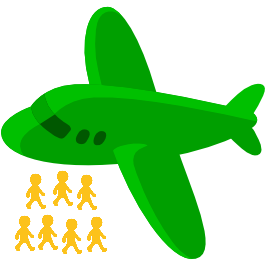
\includegraphics[width=20mm]{icons/92-emoji_android_airplane_green_withpeople.png}
\columnsend

### Miembros estáticos

\subsubtitleB{Operaciones estáticas:}

- Una clase puede definir algunas operaciones como \bld{\texthigh{estáticas}}:

\buildrboxx[0.9\textwidth]{}

- Las instancias \texthigh{no tienen acceso} a esa operación.
- Pasa a ser una operación \texthigh{propia de la clase}.
- El resultado ---y la manera de obtenerlo--- no dependen de las particularidades de ninguna instancia de la clase.

\finishrboxx

### Miembros estáticos

\subsubtitleB{Operaciones estáticas:}

- Hay clases que definen casi todas sus operaciones como estáticas:
    - En Java, la clase \texttt{Math} provee funciones matemáticas.
    - Calcular la tangente de un ángulo, o determinar el menor entre dos números, no son
    operaciones que dependan de alguna circunstancia en particular.
        - No existen ``distintas versiones de la matemática'' que las implementen de manera
        diferenciada.

\columnsbegin
\column{0.1\textwidth}
\column{0.4\textwidth}
\centering
\includegraphics[width=15mm]{icons/113-emoji_android_heavy_plus_sign.png}
\column{0.4\textwidth}
\centering
\includegraphics[width=15mm]{icons/100-emoji_android_heavy_multiplication_x.png}
\column{0.1\textwidth}
\columnsend

### Miembros estáticos

\subsubtitleB{Operaciones estáticas: ejemplo}

\columnsbegin
\column[T]{0.6\textwidth}

- Tenemos una clase que representa órdenes de compra.
    - Cada vez que ingresa una nueva orden, creamos un objeto.
    - Entre sus atributos, las órdenes tienen un código identificador único.
        - ¿De dónde lo obtienen?

\column[T]{0.4\textwidth}

\centering
\includegraphics[width=20mm]{icons/546-emoji_android_package.png}

\pause

\vspace{3em}

\tikzinlinec[0.5]{%
    \umlclass[x=0,y=0]{OrdenDeCompra}
        {--id : integer\\--cliente : Cliente}%
        {\umlstatic{+nuevoId() : integer}}
}

\columnsend

# Ejemplos de implementación en Java

## Ejemplos de implementación en Java

### Implementar una clase simple {.fragile}

\subsubtitleB{Dos clases ya vistas:}

\columnsbegin

\column{0.5\textwidth}

\tikzinlinec[0.5]{%
    \umlclass[x=0,y=0]{Vuelo}%
      {--númDeVuelo : Integer\\ --horaSalida : Date\\ --duraciónVuelo : Integer}%
      {+atrasarVuelo(Integer) : Date\\ +obtHoraLlegada() : Date}
}

\column{0.5\textwidth}

\vspace{-2em}
\begin{lstlisting}
public class Vuelo {
    private int numDeVuelo;
    private Date horaSalida;
    private int duracionVuelo;

    public Date atrasarVuelo(int atraso) {
        // acciones
    }

    public Date obtHoraLlegada() {
        // acciones
    }
}
\end{lstlisting}

\columnsend

\columnsbegin

\column{0.5\textwidth}

\tikzinlinec[0.5]{%
    \umlclass[x=8,y=0]{CuentaBancaria}%
      {--dueño : Cliente\\ --balance : Money\\ --apertura : Date}%
      {+depositar(monto : Money) : Boolean\\ +sacar(monto : Money) : Boolean}
}

\column{0.5\textwidth}

\vspace{-1em}
\begin{lstlisting}
public class CuentaBancaria {
    private Cliente duenno;
    private Money balance;
    private Date apertura;

    public boolean depositar(Money monto) {
        // acciones
    }

    public boolean sacar(Money monto) {
        // acciones
    }
}
\end{lstlisting}

\columnsend

### Implementar una asociación {.fragile}

- Ahora implementemos una asociación entre tres clases.
- Primero veamos esta asociación mediante un diagrama de dominio:

\tikzinlinec{
    \umlclass[x=-7,simple]{Estudiante}{}{}
    \umlclass[x=0,simple]{Curso}{}{}
    \umlclass[x=7,simple]{Profesor}{}{}
    \umlassoc[mult1=5..60,pos1=0.1,mult2=*,pos2=0.9,name=toma]{Estudiante}{Curso}
    \umlassoc[mult1=0..3,pos1=0.1,mult2=1,pos2=0.9,name=dicta]{Curso}{Profesor}
    % \umlassoc[mult1=*,pos1=0.1,mult2=1,pos2=0.9,name=especifica]{Producto}{DescProd}
    \draw (toma-1) {} node[above=1mm] (toma) {toma};
    \draw [-triangle 45,above=1mm] (toma.east)+(0.2,0) -- ++(0.3,0);
    \draw (dicta-1) {} node[above=1mm] (dicta) {dicta};
    \draw [-triangle 45,above=1mm] (dicta.west)+(-0.2,0) -- ++(-0.3,0);
}

- Una implementación sería la siguiente:
    - No olvidar que hemos omitido todo el código no relevante.

\columnsbegin

\column{0.27\textwidth}

\begin{lstlisting}
public class Estudiante {
    /** attributos omitidos */
    private Curso[] listaCursos;

    /** métodos omitidos */
}
\end{lstlisting}

\column{0.05\textwidth}

\column{0.36\textwidth}

\begin{lstlisting}
public class Curso {
    /** attributos omitidos */
    private Estudiante[] listaAlumnos;
    private Profesor profesor;

    /** métodos omitidos */
}
\end{lstlisting}

\column{0.05\textwidth}

\column{0.27\textwidth}

\begin{lstlisting}
public class Profesor {
    /** attributos omitidos */
    private Curso[] listaCursos;

    /** métodos omitidos */
}
\end{lstlisting}
\columnsend

### Relación entre D.C. y D.S.

\subsubtitleB{Entre los diagramas de clases y de secuencia tenemos:}

- Ya sabemos que los objetos no son entes estáticos.
    - No solamente guardan datos o propiedades de cada instancia.
    - También \bld{interactúan} entre sí o con instancias de otras clases.

- La interacción se lleva a cabo a través de \alert{mensajes}.
    - Una instancia, al recibir un mensaje, la procesa mediante una operación (implementada en
    un método).
    - Al conjunto de mensajes que una instancia pueda antender, se le denomina \alert{interfaz}.
        - \bld{Ojo} con los distintos usos de la palabra interfaz.


### Ejemplo: adm. propiedades

\subsubtitleB{Introducción}

- Analizaremos un caso de una administradora de propiedades.
- En particular:
    - El proceso de agregar un inmueble (Casa o Depto) al sistema.
- Lo veremos en tres fases:
    1. Un \bld{diagrama de clases} parcial.
    1. Un \bld{diagrama de secuencia de sistema} con la interacción de un usuario con el sistema.
    1. Un \bld{diagrama de clases} que incorpore la interacción ya descrita.

### Ejemplo: adm. propiedades

\subsubtitleB{Modelos iniciales}

- Consideremos el siguiente modelo parcial:

\tikzinlinec[0.55]{%
    \exAdmProps
}

### Ejemplo: adm. propiedades

\subsubtitleB{Modelos iniciales}

- Y consideremos el siguiente diagrama de secuencia:

\tikzinlinec[0.5]{
    \begin{umlseqdiag}
    \umlactor[no ddots,x=0]{Usuario}
    \umlbasicobject[x=8]{Sistema}
    \begin{umlcall}[op={datosInmueble(id,año,dir,nombre,rut)}]{Usuario}{Sistema}
    \end{umlcall}
    \begin{umlfragment}[type=alt,label=si es casa,inner xsep=8]
        \begin{umlcall}[op={datosCasa(patio)},dt=7]{Usuario}{Sistema}
        \end{umlcall}
        \umlfpart[si es depto]
        \begin{umlcall}[op={datosDepto(np, nd)},dt=5]{Usuario}{Sistema}
        \end{umlcall}
    \end{umlfragment}
    \begin{umlcall}[op=concretarIngreso(),return=Confirmación]{Usuario}{Sistema}
    \end{umlcall}
    \end{umlseqdiag}
}

### Ejemplo: adm. propiedades

\subsubtitleB{Incorporar interacción con sistema}

Representemos en el D.C. la interacción entre un usuario y el sistema vista en el D.S. anterior:

\tikzinlinec[0.45]{%
    \exAdmPropsInteraction
}

### Ejemplo: adm. propiedades

\subsubtitleB{Comentarios}

- Fijarse la manera en que cada tipo de asociación se refleja en el código final.
- ¿Por qué hay una dependencia entre \texthigh{AdmPropiedades} tanto con \texthigh{Casa} como
con \texthigh{Departamento}?
    - ¿Por qué esta dependencia no se dibuja entre \texthigh{AdmPropiedades} e \texthigh{Inmueble}?
- En el diagrama anterior se podría haber incluido una \texthigh{interfaz} que fuera implementada
por la clase \texthigh{AdmPropiedades}.
    - ¿Por qué?
- ¿Está bien crear una instancia de \texthigh{Propietario} tal como lo hicimos?

### Ejemplo: adm. de órdenes de compra

\subsubtitleA{Propuesto:}{¿Qué diagrama de secuencia podrían imaginarse para este modelo?}

\tikzinlinec[0.45]{%
    \umlclass{Cliente}{--nombre : String}{}
    \umlclass[x=8]{Orden}{--fecha : Date\\--estado : int}{+calcImpuesto() : double\\+calcTotal() : double}
    \umlclass[x=5,y=-4]{Pago}{--monto : double}{}
    \umlclass[x=0,y=-9]{Crédito}{--numTarj : String\\--tipo : int\\--expiracion : Date}{+validar() : boolean}
    \umlclass[x=5,y=-9]{Efectivo}{}{}
    \umlclass[x=10,y=-9]{Cheque}{--titular : String\\--banco : String}{+validar() : boolean}
    \umlclass[x=17]{DetalleOrden}{--cantidad : int}{+calcSubTotal() : double\\+calcPeso() : double}
    \umlclass[x=17,y=-8]{Item}{--peso : double\\--descripcion : String}{+calcPeso() : double}
%
    \umlVHVinherit[anchor2=-120]{Crédito}{Pago}
    \umlVHVinherit[anchor2=-90]{Efectivo}{Pago}
    \umlVHVinherit[anchor2=-60]{Cheque}{Pago}
    \umlaggreg[attr1=|1,attr2=itemLinea|1..*]{Orden}{DetalleOrden}
    \umlassoc[attr1=|1,attr2=|*]{Cliente}{Orden}
    \umlVHuniassoc[anchor1=-70,arg1=1,arg2=1..*,pos2=1.8]{Orden}{Pago}
    \umluniassoc[attr1=|*,attr2=|1,pos1=0.1,pos2=0.9]{DetalleOrden}{Item}
}

